\appendix 
\chapter{\label{sec:appendixA}}
\begin{figure}[htbp]
	\centering % Centers the image and caption
	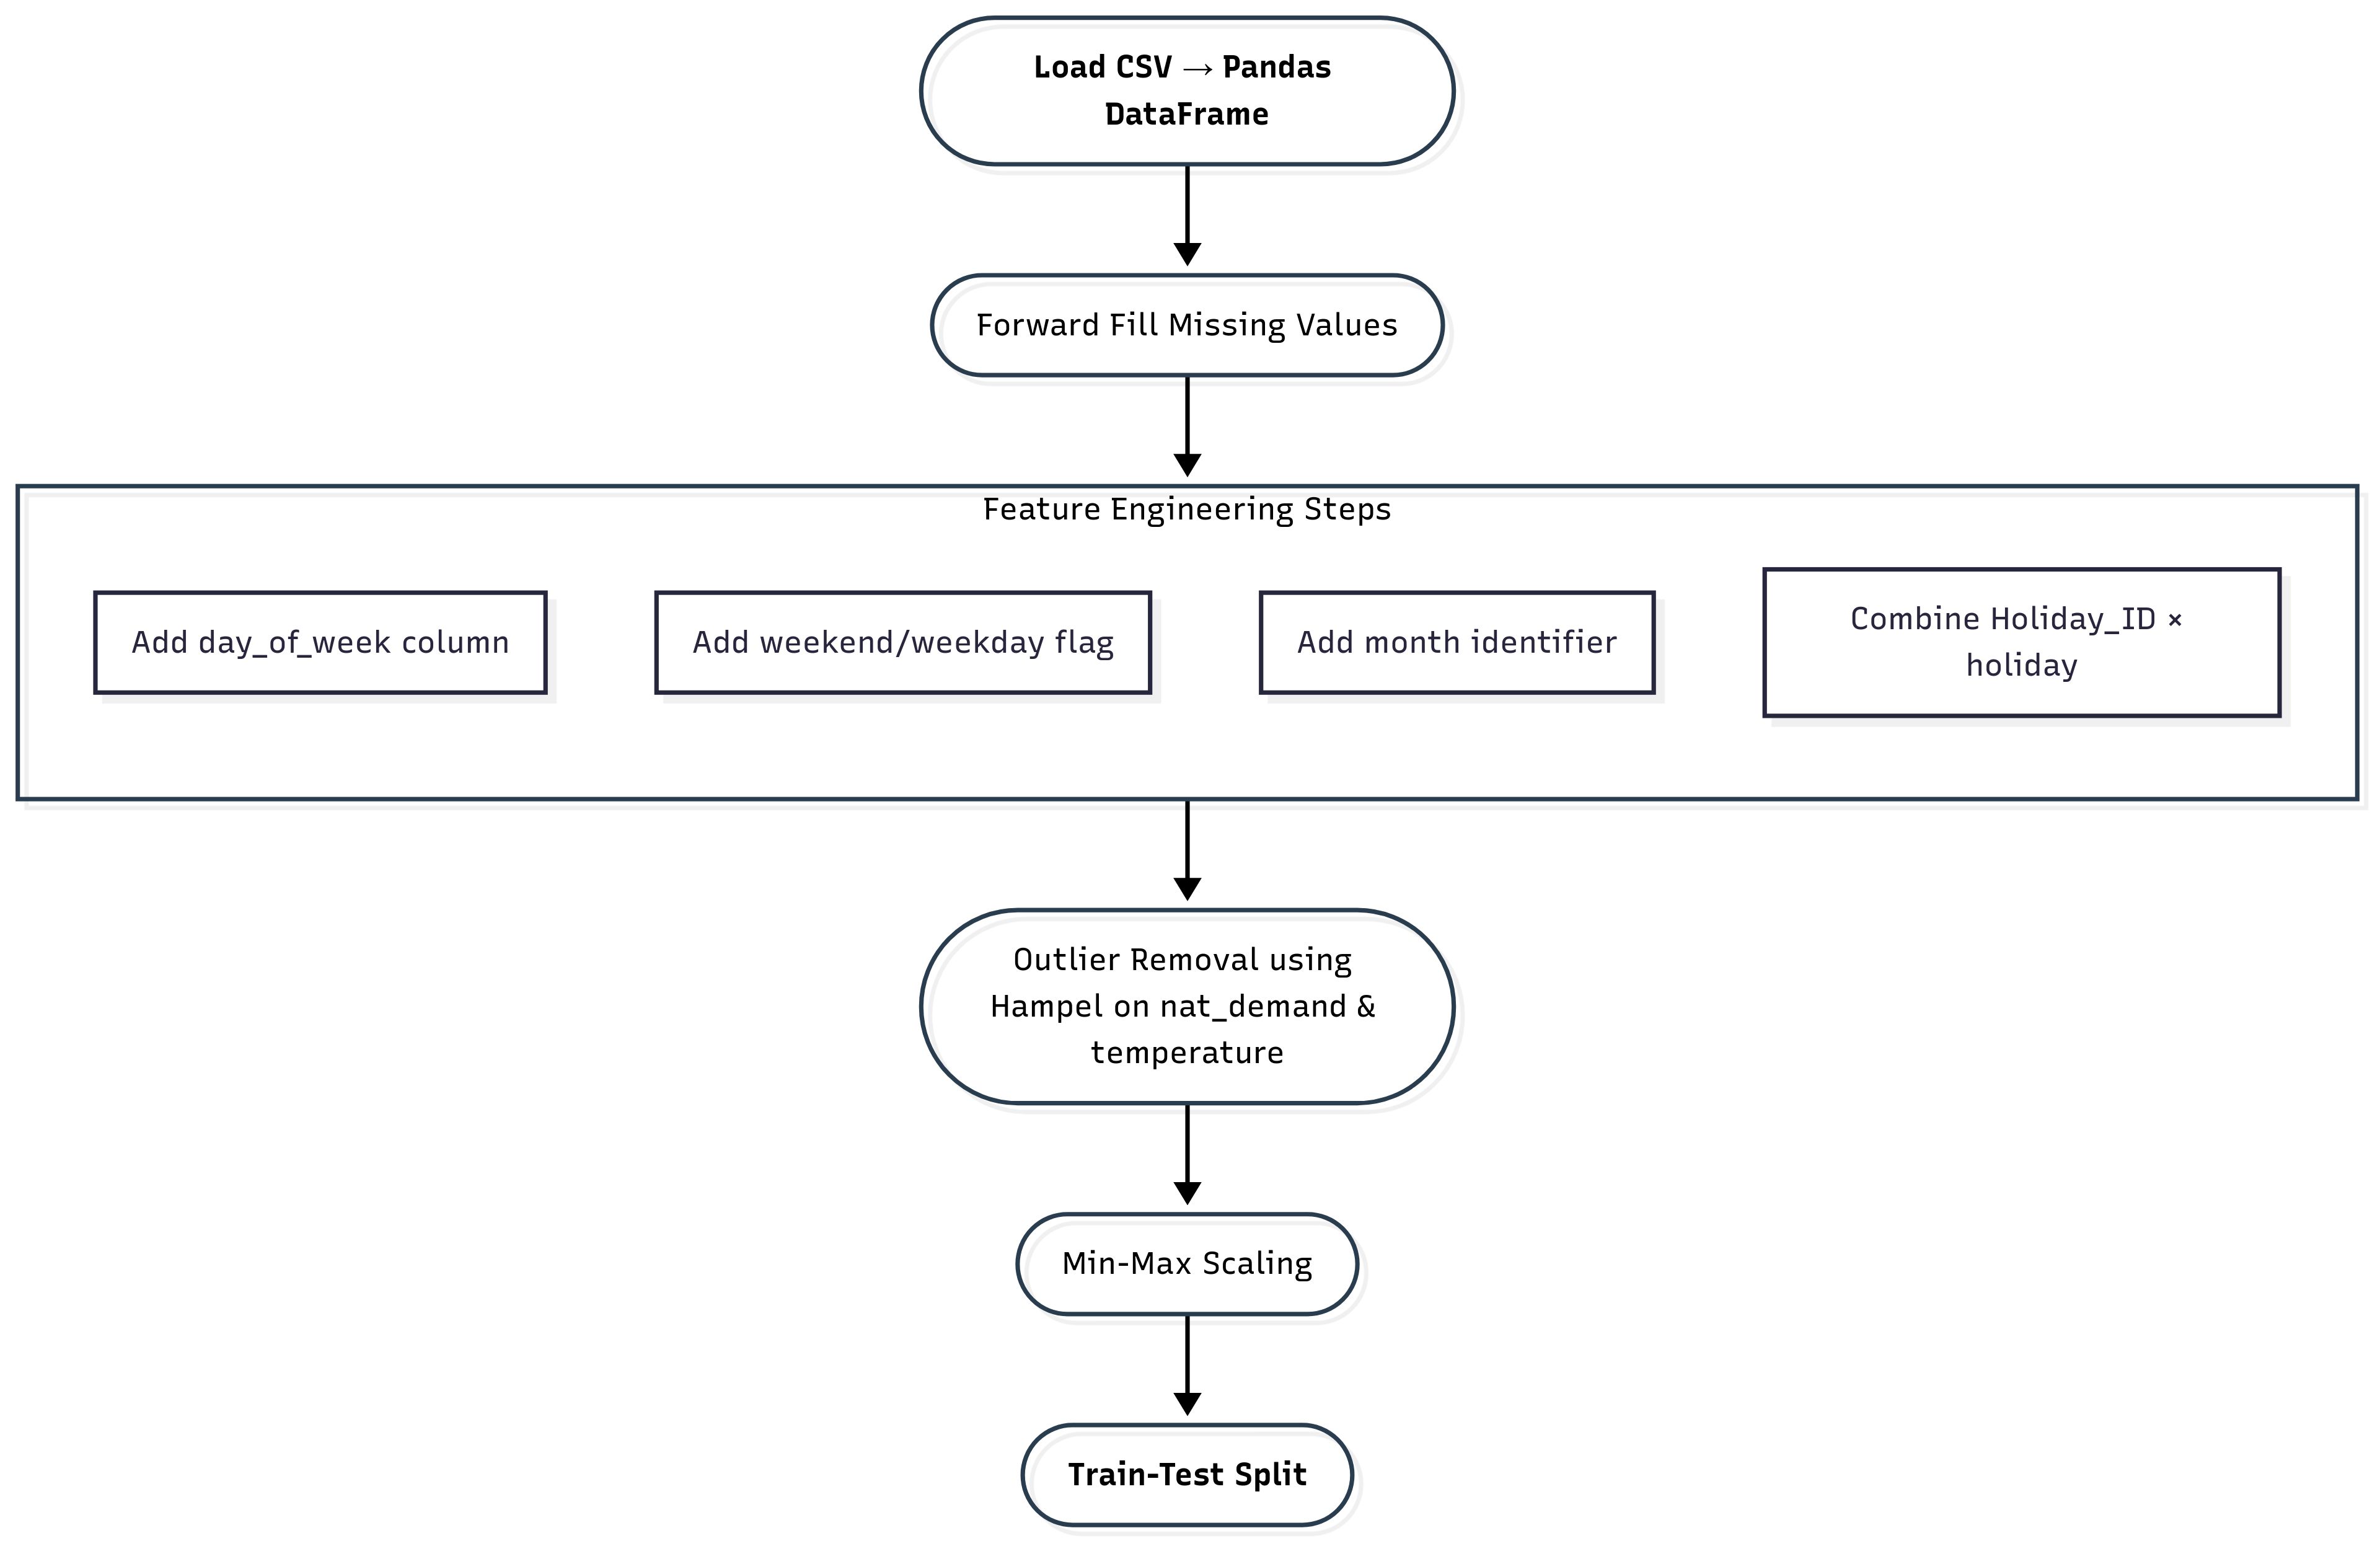
\includegraphics[scale=0.1]{Chapters/images/preprocess.png}
	\caption{The data preprocessing steps taken to process the data for model training}
	\label{fig:preprocessing_steps_flowchart} % For referencing the figure later
\end{figure}


\begin{figure}[htbp]
	\centering % Centers the image and caption
	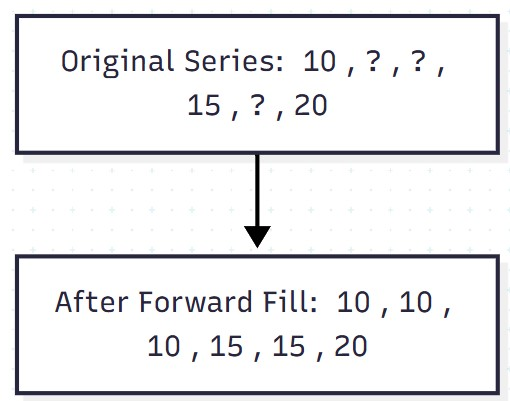
\includegraphics[scale=0.4]{Chapters/images/forward_fill.jpg}
	\caption{Forward Fill algorithm demonstration}
	\label{fig:forward_fill} % For referencing the figure later
\end{figure}
\begin{figure}[h]
	\centering
	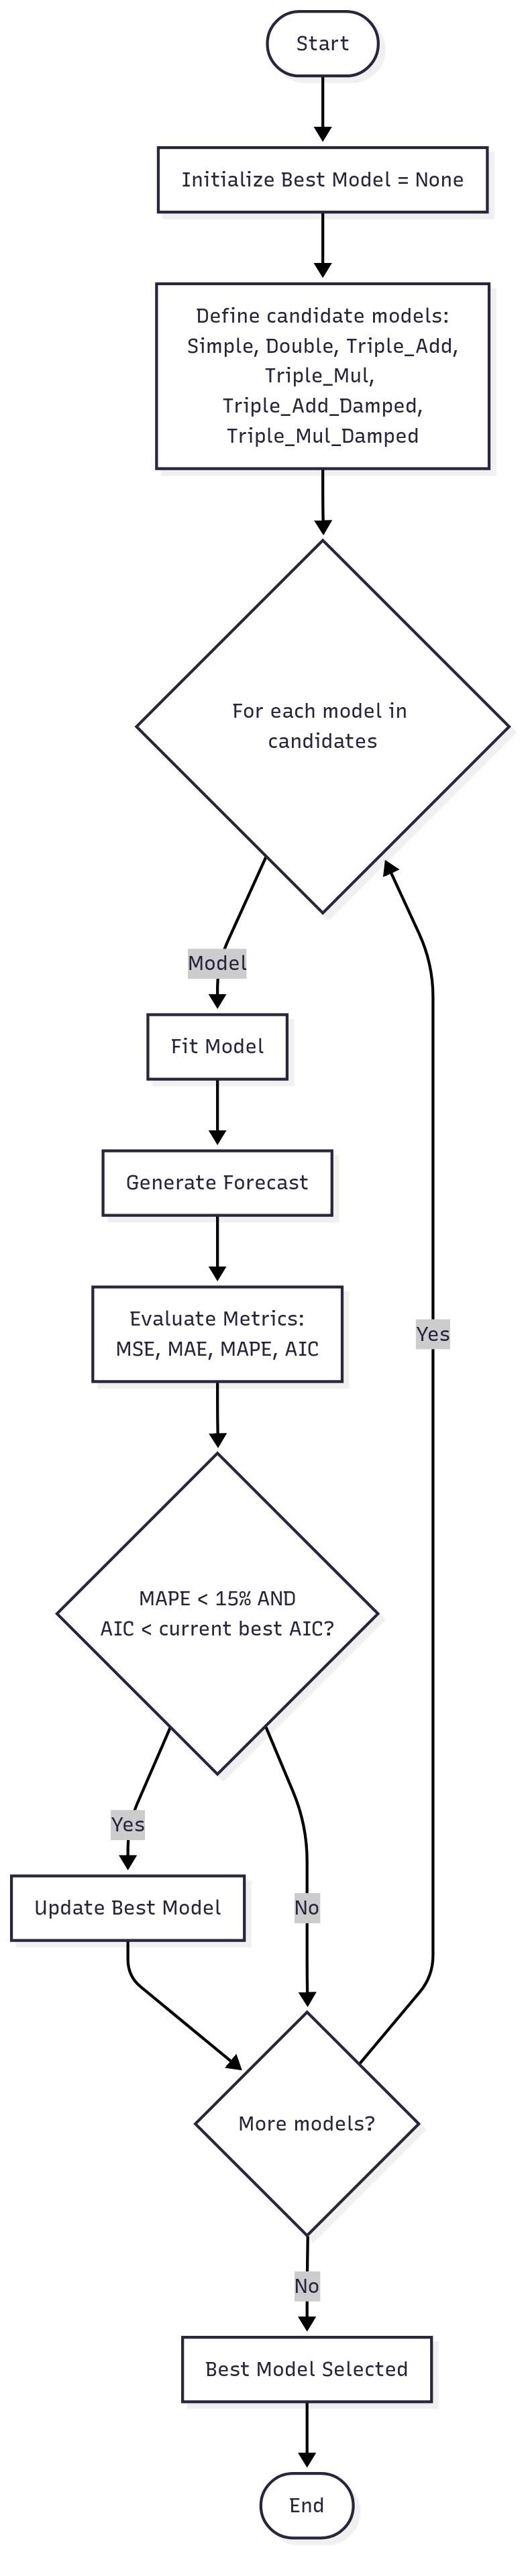
\includegraphics[scale=0.18]{"Chapters/images/exponentialsmoothingmodel.png"}
	\caption{Exponential smoothing model selection design choices.}
	\label{fig:exponential-smoothing-model-choice}
\end{figure}

\begin{figure}[h]
	\centering
	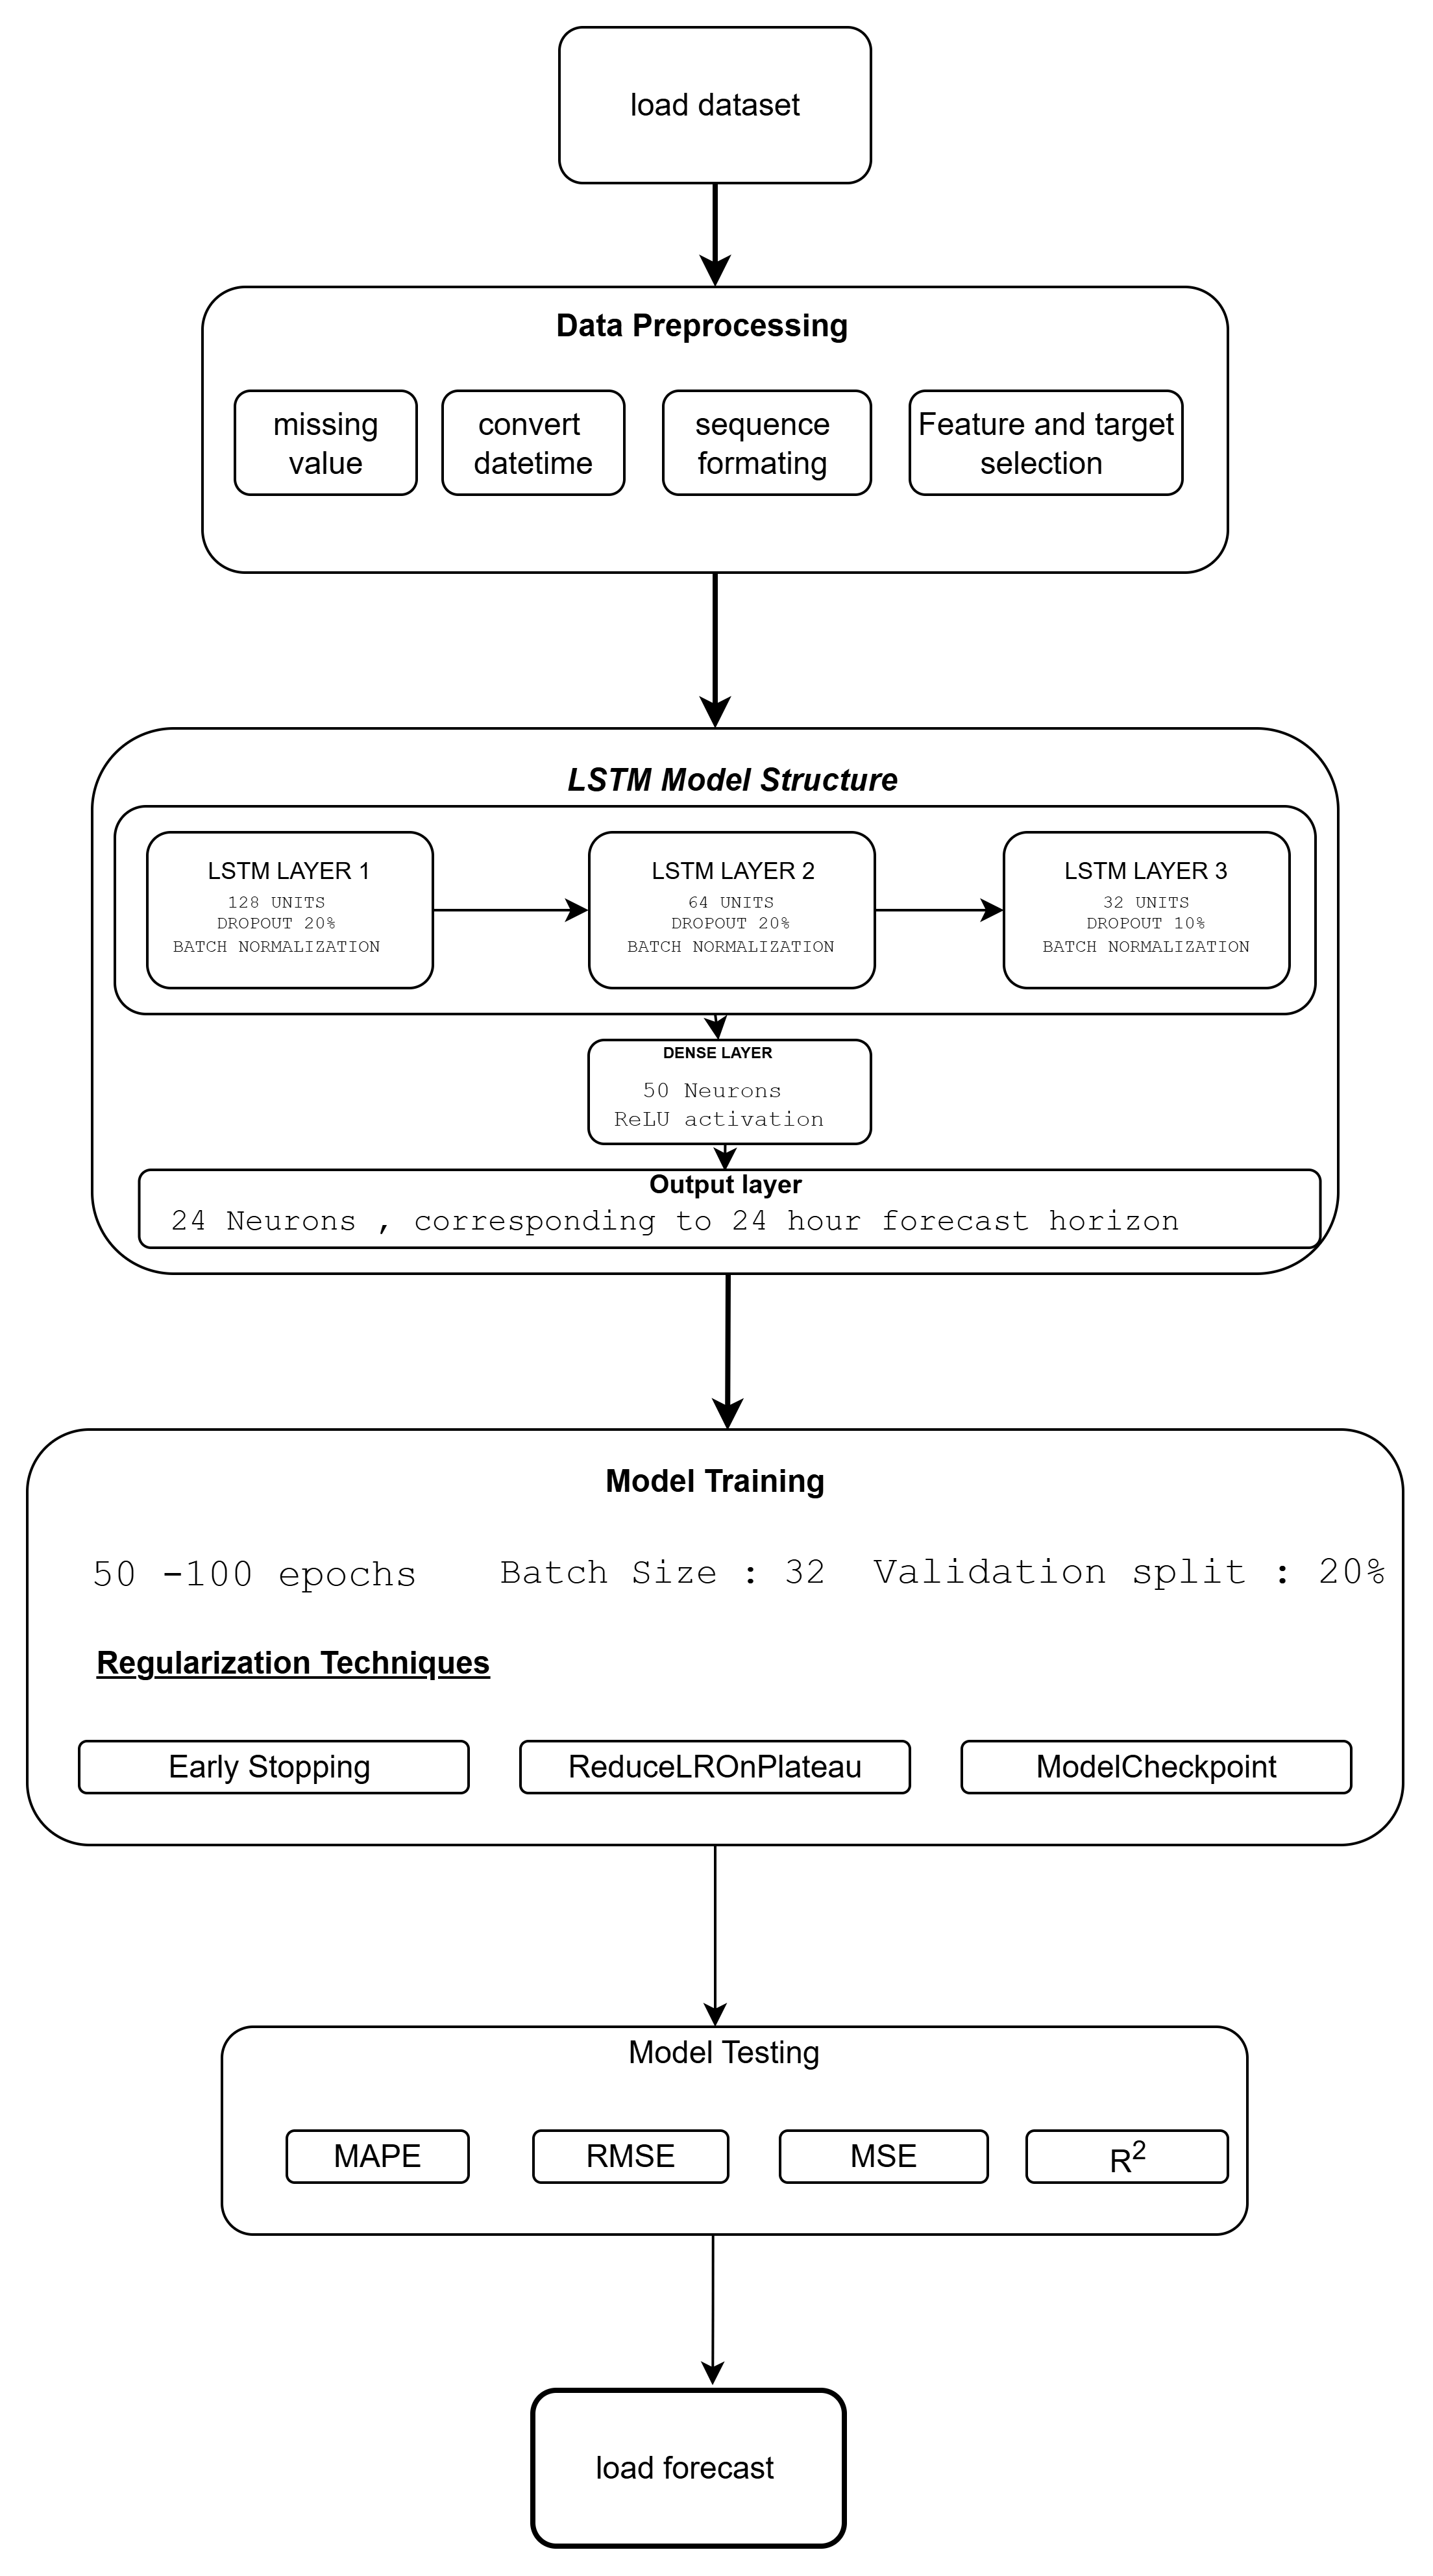
\includegraphics[width=0.7\linewidth]{Chapters/images/lstm_flowchart}
	\caption{full flowchart of the lstm model}
	\label{fig:lstmflowchart}
\end{figure}
